\documentclass[11pt, oneside]{article}   	% use "amsart" instead of "article" for AMSLaTeX format
\usepackage{geometry}                		% See geometry.pdf to learn the layout options. There are lots.
\geometry{letterpaper}                   		% ... or a4paper or a5paper or ... 
%\geometry{landscape}                		% Activate for for rotated page geometry
%\usepackage[parfill]{parskip}    		% Activate to begin paragraphs with an empty line rather than an indent
\usepackage{graphicx}				% Use pdf, png, jpg, or eps� with pdflatex; use eps in DVI mode
								% TeX will automatically convert eps --> pdf in pdflatex		
\usepackage{amssymb}
\usepackage{amsmath}
\usepackage{parskip}
\usepackage{color}
\usepackage{hyperref}

\title{Capacitor Equations}
%\author{The Author}
%\section{}
%\subsection*{}
\date{}							% Activate to display a given date or no date

\graphicspath{{/Users/telliott_admin/Dropbox/Tex/png/}}
% \begin{center} 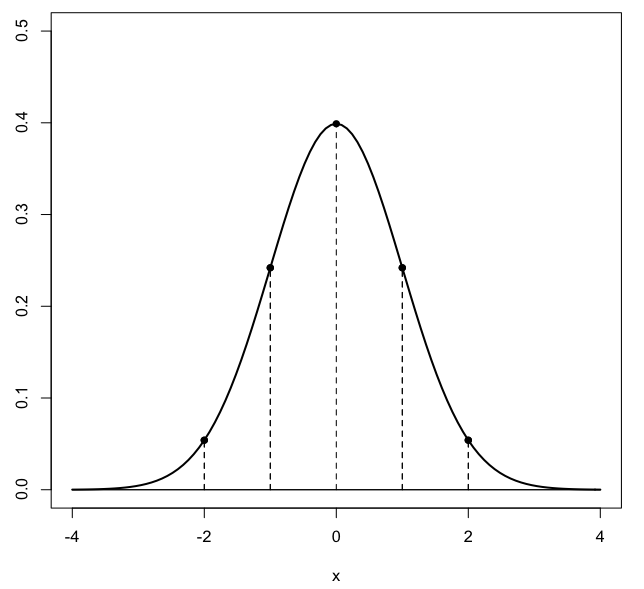
\includegraphics [scale=0.4] {gauss3.png} \end{center}
\begin{document}
\maketitle
\Large
A capacitor consists of two charged objects (parallel plates, or concentric sphere and shell).  For the (infinite) parallel plates example, we verified previously the formula
\[ E = \frac{\sigma}{\epsilon_0} \]
This result is easy to see if we visualize an electric field with lines of flux.  By symmetry, there is nowhere to go for a line that leaves the positive plate but directly toward the negative plate.  There is no way for the lines to spread out with distance, hence, no dependence on the separation.

For a finite capacitor, if we ignore edge effects, the same basic result holds.  We compute the potential difference, or voltage, between two plates as
\[ V = Ea \]
The voltage difference does depend on the distance separating the plates.  Now since $\sigma = Q/A$
\[ V = Ed = \frac{Qa}{\epsilon_0 A} = \frac{Q}{C} \]
where $C$ is defined to be
\[ C = \frac{\epsilon_0 A}{a} \]
Capacitance $C$ relates voltage to charge
\[ CV = Q \]
\[ V = \frac{Q}{C} \]
The higher the capacitance, the smaller the voltage for a given amount of stored charge.  The permittivity $\epsilon_0$ changes the $\epsilon$ for other materials, where $\epsilon = k \epsilon_0$.  For example, for paper, $k=3.5$ or so.

\subsection*{energy}
If we consider a capacitor with a charge $Q$ on it, and evaluate the work done in bringing a small amount of positive charge $dQ$ to the positively charged plate, work is equal to force times distance so
\[ dW = E a \ dq = V \ dq \]
\[ W = \int dW = \int V \ dq = \int \frac{Q}{C} \ dq \]
Hence, in building up a charge $Q$ on a capacitor the work done is 
\[ W = \frac{Q^2}{2C} = \frac{(CV)^2}{2C} = \frac{1}{2}CV^2 \]

\subsection*{discharge circuit}
Consider a resistor $R$ and a capacitor $C$, and a switch.  The capacitor is initially charged.  Close the switch and what happens?  Use the standard rules and go around the circuit looking at the voltage drops across the components.  We get
\[ \frac{Q}{C} - IR = 0 \]
If current is defined as $I = - dq/dt$, then
\[ \frac{Q}{C} = IR = -\frac{dq}{dt} R \]
\[ \frac{dq}{Q} = -\frac{1}{RC} dt \]
\[ Q = Q_0 e^{-t/RC} \]
And the current is
\[ I = - \frac{dq}{dt} = \frac{1}{RC} Q_0 e^{-t/RC} \]
The charge decays exponentially with time with characteristics governed by $RC$.  In particular, if $Q = Q_0/2$ then
\[ \ln 2 = \frac{T_{1/2}}{RC} \]

\subsection*{energy}
On the other hand,onsider a circuit containing a battery (or EMF $\mathcal{E}$), a resistor $R$ and a capacitor $C$, and a switch.  The capacitor is initially uncharged.  Close the switch and what happens?  Use the standard rules and go around the circuit looking at the voltage

\subsection*{series and parallel}
Everyone has probably seen the equations for resistors.
\[ V = IR \]
Put two resistors in series, and each one must carry the full current, but the voltage drop is distributed, part of it over each resistor separately.  Hence:
\[ V_{tot} = V_1 + V_2 = IR_1 + IR_2 \]
\[ = I(R_1 + R_2) = I R_{e} \]
where $R_e$ is the equivalent resistance for the two resistors together.
\[ R_1 + R_2 = R_e \]
In contrast, if the resistors are in parallel, they have the same voltage drop and the current is distributed.
\[ I = \frac{V}{R} \]
\[ I = I_1 + I_2 =  \frac{V}{R_e} \]
Thus
\[ \frac{V}{R_e} = \frac{V}{R_1} + \frac{V}{R_2} \]
\[ \frac{1}{R_e} = \frac{1}{R_1} + \frac{1}{R_2} \]
Resistances add in series, and their reciprocals add, in parallel.

Capacitors are just the opposite.  Capacitance is additive in parallel, but the reciprocals add in series.
\begin{center} 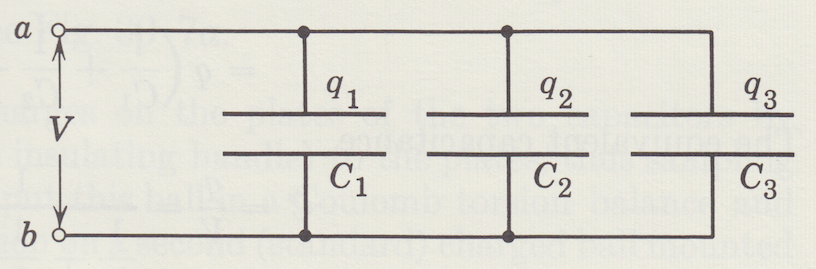
\includegraphics [scale=0.4] {capacitor_parallel.png} \end{center}
In parallel, both components have the same voltage, but the charge is additive.
\[ V = \frac{Q_1}{C_1} \]
\[ V = \frac{Q_2}{C_1} \]
\[ Q_{tot}= C_e V = C_1 V + C_2 V \]
Thus
\[ C_e = C_1 + C_2 \]

In series, the charge is the same and the voltages add
\[ V_{tot} = \frac{Q}{C_1} + \frac{Q}{C_2} = \frac{Q}{C_e} \]
\[ \frac{1}{C_1} + \frac{1}{C_2} = \frac{1}{C_e} \]


\end{document}  